\documentclass[12pt, leqno]{article} %% use to set typesize
\usepackage{fancyhdr}
\usepackage[sort&compress]{natbib}
\usepackage[letterpaper=true,colorlinks=true,linkcolor=black]{hyperref}

\input{commonm}

\newcommand{\hdr}[2]{
  \pagestyle{fancy}
  \lhead{Bindel, Fall 2019}
  \rhead{Matrix Computation}
  \fancyfoot{}
  \begin{center}
    {\large{\bf HW for #1}} \\ (due: #2)
  \end{center}
  \lstset{language=matlab,columns=flexible}
}


\begin{document}

\hdr{2019-10-04}

\section{QR and Gram-Schmidt}

We now turn to our first numerical method for computing the
QR decomposition: the Gram-Schmidt algorithm.  This method is
usually presented in first linear algebra classes, but is
rarely interpreted as a matrix factorization.  Rather, it is
presented as a way of converting a basis for a space into an
orthonormal basis for the same space.  If $a_1, a_2, \ldots, a_n$
are column vectors, the Gram-Schmidt algorithm is as follows:
for each $j = 1, \ldots, n$
\begin{align*}
  \tilde{a}_j &= a_j - \sum_{i=1}^{j-1} q_i q_i^T a_j \\
  q_j &= \tilde{a}_j / \|\tilde{a}\|_j.
\end{align*}
At the end of the iteration, we have that the $q_j$ vectors are
all mutually orthonormal and
\[
  \operatorname{span}\{ a_1, \ldots, a_j \} =
  \operatorname{span}\{ q_1, \ldots, q_j \}.
\]
To see this as a matrix factorization, we rewrite the iteration as
\begin{align*}
  r_{ij} &= q_i^T a_j \\
  \tilde{a}_j &= a_j - \sum_{i=1}^{j-1} q_i r_{ij} \\
  r_{jj} &= \|\tilde{a}\|_j \\
  q_j &= \tilde{a}_j / r_{jj}
\end{align*}
Putting these equations together, we have that
\[
  a_j = \sum_{i=1}^j q_i r_{ij},
\]
or, in matrix form,
\[
  A = QR
\]
where $A$ and $Q$ are the matrices with column vectors $a_j$ and $q_j$,
respectively.

Sadly, the Gram-Schmidt algorithm is not backward stable.
The problem occurs when a vector $a_j$ is nearly in the span of
previous vectors, so that cancellation rears its ugly head in the
formation of $\tilde{a}_j$.  The
classical Gram-Schmidt (CGS) method that we have shown is particularly
problematic; a somewhat better alternative is the modified Gram-Schmidt
method (MGS) algorithm:
\begin{lstlisting}
  % Overwrite A with Q via MGS, store R separately
  R = zeros(n);
  for j = 1:n
    for i = 1:n-1
      R(i,j) = Q(:,i)'*A(i,j);
      A(:,j) = A(:,j) - Q(:,i)*R(i,j);
    end
    R(j,j) = norm(A(:,j));
    A(:,j) = A(:,j) / R(j,j);
  end
\end{lstlisting}
Though equivalent in exact arithmetic, the MGS algorithm has the advantage
that it computes dot products with the updated $\tilde{a}_j$ as we go
along, and these intermediate vectors have smaller norm than the original
vector.  Sadly, this does not completely fix the matter: the computed $q_j$
vectors can still drift away from being orthogonal to each other.  One can
explicitly re-orthogonalize vectors that drift away from orthogonality,
and this helps further.  In practice, though, we usually don't bother: if
backward stability is required, we turn to other algorithms.

Despite its backward instability, the Gram-Schmidt algorithm forms a very
useful building block for iterative methods, and we will see it frequently
in later parts of the course.

\section{Householder transformations}

The Gram-Schmidt orthogonalization procedure is not generally
recommended for numerical use.  Suppose we write $A = [a_1 \ldots
  a_m]$ and $Q = [q_1 \ldots q_m]$.  The essential problem is that if
$r_{jj} \ll \|a_j\|_2$, then cancellation can destroy the accuracy of
the computed $q_j$; and in particular, the computed $q_j$ may not be
particularly orthogonal to the previous $q_j$.  Actually, loss of
orthogonality can build up even if the diagonal elements of $R$ are
not exceptionally small.  This is Not Good, and while we have some
tricks to mitigate the problem, we need a different approach if we
want the problem to go away.

Recall that one way of expressing the Gaussian elimination algorithm
is in terms of Gauss transformations that serve to introduce zeros
into the lower triangle of a matrix.  {\em Householder} transformations
are orthogonal transformations (reflections) that can be used to similar
effect.  Reflection across the plane orthogonal to a unit normal
vector $v$ can be expressed in matrix form as
\[
  H = I-2 vv^T.
\]

Now suppose we are given a vector $x$ and we want to find a reflection
that transforms $x$ into a direction parallel to some unit vector $y$.
The right reflection is through a hyperplane that bisects the angle
between $x$ and $y$ (see Figure~\ref{fig1}), which we can construct
by taking the hyperplane normal to $x-\|x\|y$.  That is,
letting $u = x - \|x\|y$ and $v = u/\|u\|$, we have
\begin{align*}
  (I-2vv^T)x
  & = x - 2\frac{(x+\|x\|y)(x^T x + \|x\| x^T y)}{\|x\|^2 + 2 x^T y \|x\| + \|x\|^2 \|y\|^2} \\
  & = x - (x-\|x\|y) \\
  & = \|x\|y.
\end{align*}
If we use $y = \pm e_1$, we can get a reflection that zeros out all but the
first element of the vector $x$.  So with appropriate choices of reflections,
we can take a matrix $A$ and zero out all of the subdiagonal elements
of the first column.

\begin{figure}
\begin{center}
  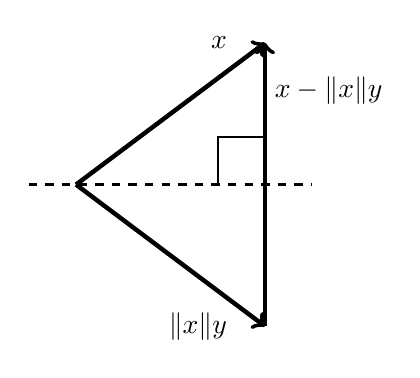
\begin{tikzpicture}[scale=0.6]
    \draw [thick,dashed] (-1,0) -- (5,0);
    \draw [ultra thick,->] (0,0) -- (4,3);
    \draw [ultra thick,->] (0,0) -- (4,-3);
    \draw [ultra thick,->] (4,-3) -- (4,3);
    \draw [thick] (3,0) -- (3,1) -- (4,1);
    \draw (4,2) node [right] {$x-\|x\| y$};
    \draw (3.4,3) node [left] {$x$};
    \draw (3.4,-3) node [left] {$\|x\| y$};
  \end{tikzpicture}
\end{center}
\caption{Construction of a reflector to transform $x$ into $\|x\|y$,
         $\|y\| = 1$.}
\label{fig1}
\end{figure}

Now think about applying a sequence of Householder transformations to
introduce subdiagonal zeros into $A$, just as we used a sequence of Gauss
transformations to introduce subdiagonal zeros in Gaussian elimination.
This leads us to the following algorithm to compute the $QR$
decomposition:
\lstinputlisting{code/hqr1.m}
Note that there are two valid choices of $u_1$ at each step;
we make the choice that avoids cancellation in the obvious version
of the formula.

As with $LU$ factorization, we can re-use the storage of $A$ by recognizing
that the number of nontrivial parameters in the vector $w$ at each step
is the same as the number of zeros produced by that transformation.
This gives us the following:
\lstinputlisting{code/hqr2.m}

If we ever need $Q$ or $Q^T$ explicitly, we can always form it from
the compressed representation.  We can also multiply by $Q$ and $Q^T$
implicitly:
\lstinputlisting{code/applyQ.m}
\lstinputlisting{code/applyQT.m}

\section{Givens rotations}

Householder reflections are one of the standard orthogonal
transformations used in numerical linear algebra.  The other standard
orthogonal transformation is a {\em Givens rotation}:
\[
  G = \begin{bmatrix}
    c & -s \\
    s & c
  \end{bmatrix}.
\]
where $c^2 + s^2 = 1$.  Note that
\[
  G = \begin{bmatrix}
    c & -s \\
    s & c
  \end{bmatrix}
  \begin{bmatrix}
    x \\ y
  \end{bmatrix} =
  \begin{bmatrix}
    cx - sy \\
    sx + cy
  \end{bmatrix}
\]
so if we choose
\begin{align*}
  s &= \frac{-y}{\sqrt{x^2 + y^2}}, &
  c &= \frac{x}{\sqrt{x^2+y^2}}
\end{align*}
then the Givens rotation introduces a zero in the second column.
More generally, we can transform a vector in $\bbR^m$ into a vector
parallel to $e_1$ by a sequence of $m-1$ Givens rotations, where
the first rotation moves the last element to zero, the second rotation
moves the second-to-last element to zero, and so forth.

For some applications, introducing zeros one by one is very
attractive.  In some places, you may see this phrased as a contrast
between algorithms based on Householder reflections and those based on
Givens rotations, but this is not quite right.  Small Householder
reflections can be used to introduce one zero at a time, too.
Still, in the general usage, Givens rotations seem to be the more
popular choice for this sort of local introduction of zeros.

\end{document}
